%Sustitucion de IEEEeqnarray
\graphicspath{ {img/BD/} }
\chapter[Background Detection of Primary User Activity in Opportunistic Spectrum Access][Background Detection of Primary User Activity in OSA]{Background Detection of Primary User Activity in Opportunistic Spectrum Access}\label{BD_chap}
\section{Introduction}\label{BD_sec_intro}
\subsection{Motivation}
One of the main problems of OSA is that current radio frequency front-ends cannot perform sensing and transmission in the same channels at the same time. 
In consequence, in OSA protocols, spectrum sensing and SU data transmission are performed in two separated phases. 
The scanning phase allows the SUs to find free channels to transmit in.
However, during the transmission phase, a channel occupied by an SU can be eventually used by a PU transmission causing a potentially harmful interference to the PU receiver.
In consequence, in OSA protocols, an SU is only allowed to transmit during a limited amount of time after which it performs a new sensing procedure (\textit{periodic spectrum sensing}).
According to a given PU activity model, the length of the SU transmission period is set to the value that maximizes the SU throughput under a given collision probability constraint. 
The generic OSA model described is referred to as \textit{optimized OSA} in this chapter, and is used as a starting point and as a benchmark for our proposal.
We propose a collision detection mechanism that performs PU activity estimation during SU packet reception, and uses it to improve the classic optimized OSA mechanism.

\subsection{Related Work}
Most of the works about collision detection for single-radio transceivers only focus on the detection carried out at the transmitter side, such as periodic spectrum sensing in OSA protocols \cite{ref:Zhou2009}, \cite{ref:Lee2008}, \cite{ref:Zhang2012_opt}. To the best of our knowledge, there are only two exceptions to this \cite{ref:Chockler05,ref:Stotas2010}. Paper \cite{ref:Chockler05} theoretically studies the impact of different receiver-side detectors, but it does not detail their implementations. The work in \cite{ref:Stotas2010} implements an energy-detector \cite[Ch. 4]{ref:Biglieri2012} at the SU Rx. However, as opposed to ours, they assume that the secondary transmission is always correctly decoded and can be substracted from the received signal.

We adopt a worst case PU QoS criteria used in previous works \cite{ref:Zhang2012_opt}, \cite{ref:Huang2009}, \cite{ref:Huang2008_opp}, by which any collision is considered to cause harmful interference to PU receivers. 
As in \cite{ref:Zhang2012_opt}, our model also includes the effect of transmission overlap in SU performance. 
Additionally, we use the statistical description of the fading in the direct and interfering links to evaluate this performance.

Perfect collision detection is implicitly assumed in \cite{ref:Zhang2013_wha,ref:Jung2012}. 
In this work, we relax that assumption, taking into consideration the multiple factors that hinder perfect detection: path loss, fading effects, and decoding probability as a function of the modulation used and the signal-to-interference-and-noise ratio. 
To overcome these difficulties and perform an optimal collision detection, the SU receiver can make use of diverse estimations performed during the successive spectrum scanning and sensing periods. 
As an example, an accurate PU traffic estimator is described in \cite{ref:Gabran2013}. 

\subsection{Our Contribution}
We refer to our proposed mechanism as \textit{background detection} (BD). 
In contrast to classic spectrum sensing, in which licensed channels are sensed while the SU transmitter is idle, the BD mechanism operates at the SU receiver during ongoing SU transmissions.
In consequence, BD uses information available at the SU receiver during packet reception to decide, by means of a Maximum \textit{A Posteriori} (MAP) estimator, if there has been an overlap in each transmission slot. 
The MAP estimator exploits existing knowledge at the SU, such as the average power of the received signals, the presence or absence of decoding errors, the PU traffic pattern, and the statistical description of the fading processes. 
Our mechanism is used simultaneously with optimized OSA, and we refer to the combined scheme as OSA-BD.
We also evaluate the robustness of the system under inaccuracies in these data.
In particular, it is shown that, while optimized OSA is very reliant on an accurate PU traffic characterization, OSA-BD achieves higher robustness against PU traffic misestimations.

The rest of this chapter is organized as follows.
Section \ref{BD_sec_system} describes the PU and SU networks and states the technical foundations of our proposal. 
Section \ref{sec:Detection} discloses the background detection mechanism, formulating the MAP rule and then computing the detection probabilities. We describe the incorporation of our idea to optimized OSA in Section \ref{sec:Markov}, and Section \ref{BD_sec_results}, contains the numerical evaluation results and comparison to benchmack schemes. Concluding remarks are written in Section \ref{BD_sec_conclusion}.

\section{System Description}\label{BD_sec_system}
\subsection{General Considerations}
\begin{figure} 
\centering
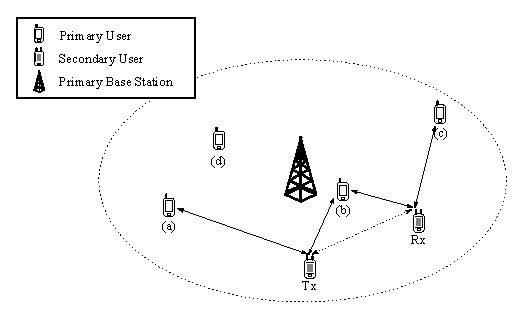
\includegraphics[scale=1]{Geo.eps}
\caption{SU pair communicating over a downlink channel of a PU BS. The SU Tx is causing interference to two PUs using the same channel. The SU Rx, equipped with our BD mechanism, is capable of detecting the signal from the PU BS while receiving the SU Tx's packets and thus, sends the SU Tx a signal to abort transmission.}\label{BD_fig_system}
\end{figure}
The mechanism proposed in this paper is very generic, and is applicable whenever the primary and the secondary wireless networks present some general characteristics described in this section.
The spectrum of the primary network is assumed to be divided into orthogonal channels.
The SUs can scan these channels to detect spectrum opportunities in them, as well as monitor PU activity and estimate the PU traffic pattern.
One type of PU access networks that fits well on this description is cellular networks, but other types may be feasible for our proposal as well.

As an example, let us consider the system in Fig. \ref{BD_fig_system}, representing the coverage area (cell) of a PU base station (PU BS), where a cognitive pair, consisting of an SU transmitter (SU Tx) and an SU receiver (SU Rx), tries to perform an SU transmission on a spectrum opportunity within this PU cell. 
It is assumed that the SU transmits in PU downlink channels. 
The BD scheme could be used for PU uplink channels as well but it would be less effective, due to possible hidden terminal problems (\textit{i.e.} a PU Tx out of range of the SU Rx detection).
Before transmitting, both the SU Tx and the SU Rx scan the licensed spectrum looking for available channels and exchange control messages containing their sensing outcomes over a dedicated control channel.
Once the cognitive pair makes the access decision, the SU Tx starts the SU transmission over one or more available channels.

The SU transmission is divided into time-slots. 
At the end of each time-slot, the SU Rx submits a control message to the SU Tx over the control channel. 
In general, this message would contain an ACK (or NACK) of the data transmitted on the time-slot.

It is assumed that the signal power received at the SU Rx remains constant during a symbol time $T_{s}$ of the SU Tx transmission. 
In this case, the probability of correct signal detection at the SU Rx is defined in terms of the probability that the signal to interference ratio (SINR) is above a given threshold, which is determined by the minimum acceptable bit error rate (BER) for correct decoding, the transmission rate and the modulation used. 
Let us consider that, given the SU data packet length, and the information and redundancy bits in it, SU packets are correctly received if the BER during the packet reception is above certain value (e.g. $10^{-3}$). 
This BER objective is attained when the ratio $E_{b}/N_{0}$ is above a threshold $\gamma_{b}$, where $E_{b}$ is the energy per bit and $N_{0}$ is the noise spectral density (including both thermal and interference noise). The threshold depends on the modulation used (e.g. for BPSK, BER = $10^{-3}$ for $\gamma_{b}=7$ dB). 
Therefore, the threshold in terms of SINR is given by $\gamma = \gamma_{b}/(BT_{b})$ where $B$ is the channel bandwidth and $T_{b}$ the bit duration.

\subsection{Principles of the Background Detection Scheme}
Each SU data packet may be received at the SU Rx with or without PU interference. 
Let $P$ denote the signal power at the SU Rx during the reception of an SU data packet. 
The SU signal is received with power $Y$ at the SU Rx and, in case of transmission overlap, the signal transmitted by the PU BS is received with power $X$ at the SU Rx. 
Let $N$ denote the average white noise power in the channel bandwidth at the SU Rx during the packet reception.
Note that $P$, $X$, and $Y$ are random variables, while $N$ is a constant determined by the noise factor of the receiver, which is a known design parameter. Therefore, we can subtract $N$ from the power observation.
Then, under PU-SU transmission overlap, $P=X+Y$ and, in absence of overlap, $P=Y$. 
Similarly, $\text{\ttfamily{SINR}}=\frac{Y}{N+X}$, with overlap, and $\text{\ttfamily{SINR}}=\frac{Y}{N}$ without overlap.
If $\text{\ttfamily{SINR}}>\gamma$ the packet is correctly received and, if $\text{\ttfamily{SINR}}\leq\gamma$ the packet is impossible to decode (error event). 

After the reception of an SU data packet, the SU Rx can obtain two observations: $P$, and the occurrence (or absence) of an error event. The idea of the background detection (BD) mechanism is to use these observations to allow the SUs estimate the presence of PU activity during SU transmissions. If PU activity is detected, the OSA algorithm may decide to end the ongoing SU transmission to protect from interference any PU terminal in range of the SU Tx (in Fig. \ref{BD_fig_system}, the PU terminals pointed by a dashed arrow) in case any of them is receiving PU BS transmissions on the channel where the overlap was detected.

The BD scheme is essentially a binary hypothesis testing mechanism conducted during SU transmission to decide on the most feasible value of a random variable $\Theta$, which takes two possible values $\left\{0,1\right\}$ at each SU packet reception. The event $\Theta = 1$ indicates that there has been PU interference during the packet reception, and $\Theta = 0$ indicates that the reception was free of PU interference.
%whether or not there has been PU interference during the reception of an SU data packet. These two hypotheses are referred to as $H_{1}$ (PU activity) and $H_{0}$ (no PU activity). 
The probability density functions (PDF) of $Y$ and $X$ are $f_{Y}(y)$ and $f_{X}(x)$ respectively. In case that both the SU Tx and the PU BS signals experience Rayleigh fading over their respective links to the SU Rx, we have $f_{Y}(y) = \displaystyle\frac{1}{p_{ss}}e^{-\frac{y}{p_{ss}}}$, and $f_{X}(x) = \displaystyle\frac{1}{p_{ps}}e^{-\frac{x}{p_{ps}}}$, where $p_{ss}$ is the average power received from the SU Tx and $p_{ps}$ is the average power received from the PU BS. Both distributions, as well as the average powers can be obtained from the previous sensing history of the SUs. 
Similarly, this sensing history provides information about the PU traffic profile and intensity on the scanned channels.
One basic metric is the probability of PU activity during the transmission time of an SU packet ($\mathbf{P}\left(\Theta = \theta\right)$), with $\theta \in \left\{0,1\right\}$.
Therefore, assuming $f_{Y}(y)$, $f_{X}(x)$ and $\mathbf{P}\left(\Theta = \theta\right)$ are known, the hypothesis testing is based on Bayesian estimation, resulting in a maximum a posteriori probability (MAP) decision rule. In Section \ref{BD_sec_results} we evaluate the sensitivity of the BD mechanism to the inaccuracies in the estimation of the PDFs and traffic parameters.

Summarizing, once the SU transmission has started, the SU Rx obtains, upon each packet reception, the following observation:
\begin{equation}
\left(P,E\right) = 
\begin{cases}
\left(p_{r},0\right) &,\mbox{if }\text{\ttfamily{SINR}}>\gamma\\
\left(p_{r},1\right) &,\mbox{if }\text{\ttfamily{SINR}}\leq\gamma
\end{cases}
\end{equation}
And, upon this observation, the MAP decision rule selects the hypothesis having the maximum posterior distribution over the two possible values of $\theta$. Next section provides a detailed derivation for the BD MAP rule, and obtains the probabilities of correct and incorrect detection of the MAP estimator.

\section{PU Activity Detection in Background}\label{sec:Detection}
\subsection{MAP Rule}\label{sec:MAPrule}
Given the observation $\left(P=p_{r},E=e\right)$, the MAP rule selects the hypothesis $H_{i}$ for which the \textit{a posteriori} probability $\mathbf{P}\left(\Theta=\theta|P=p_{r},E=e\right)$ is largest. 
By Bayes' rule this is equivalent to selecting the hypothesis maximizing $p_{\Theta}\left(\theta\right)f_{P,E|\Theta}\left(p_{r},e|\theta\right)$.
Because $E$ is a discrete random variable, we have to consider separately each of its possible values ($E=0$ if the SU packet is received without errors and $E=1$ otherwise) for the computation of the \textit{a posteriori} probability. 
Let $E_{0}$ and $E_{1}$ refer to the events $E=0$ and $E=1$, respectively. Similarly, we use $H_{0}$ and $H_{1}$ to refer to the events $\Theta=0$ and $\Theta=1$. 
Let us derive the expression of $f_{P,E|\Theta}\left(p_{r},e|\theta\right)$ for each possible combination of $E_{0}$ and $E_{1}$ with $H_{0}$ and $H_{1}$.
\subsubsection{Case $E_{1}$, $H_{1}$} Applying the definitions we have
\begin{equation}\label{definitionE1H1}
\begin{array}{lcl}
f_{P,E_{1}|H_{1}}\left(p_{r},E_{1}|H_{1}\right) & = & \displaystyle\frac{\partial}{\partial p_{r}}\mathbf{P}\left(P\leq p_{r},\text{\ttfamily{SINR}} \leq \gamma | H_{1}\right)\\
&= & \displaystyle\frac{\partial}{\partial p_{r}}\mathbf{P}\left(X+Y\leq p_{r},Y\leq N\gamma+X\gamma\right)
\end{array}
\end{equation}
We will first find the joint PDF of $P$ and $X$ and then integrate to find the PDF of $P$.
\begin{equation}\label{PxE1H1}
\begin{array}{lcl}
\mathbf{P}\left(X+Y\leq p_{r},Y\leq N\gamma+X\gamma|X=x\right) & = & \mathbf{P}\left(Y\leq p_{r}-x,Y\leq N\gamma+x\gamma|X=x\right)\\
& = &\mathbf{P}\left(Y\leq \text{min}\left(p_{r}-x,N\gamma+x\gamma\right)|X=x\right)\\
& = &\mathbf{P}\left(Y\leq \text{min}\left(p_{r}-x,N\gamma+x\gamma\right)\right)\\
& = & \displaystyle\int_{-\infty}^{\text{min}\left(p_{r}-x,N\gamma+x\gamma\right)}f_{Y}(y)dy\\
& = &
\begin{cases}
\displaystyle\int_{-\infty}^{p_{r}-x}f_{Y}(y)dy &,\mbox{if }p_{r}\leq N\gamma+x\left(\gamma+1\right)\\
\displaystyle\int_{-\infty}^{N\gamma+x\gamma}f_{Y}(y)dy &,\mbox{otherwise }
\end{cases}
\end{array}
\end{equation}
where the third equality comes from the independence of the PU and SU signals, $X$ and $Y$. By differentiating both sides with respect to $p_{r}$ we obtain
\begin{equation}\label{fxE1H1}
f_{P,E_{1}|H_{1},X}\left(p_{r},E_{1}|H_{1},x\right) =
\begin{cases}
f_{Y}\left(p_{r}-x\right) &,\mbox{if }p_{r}\leq N\gamma+x\left(\gamma+1\right)\\
0 &,\mbox{otherwise }
\end{cases}
\end{equation}
Then, the joint PDF of $P$ and $X$ is
\begin{equation}\label{jointE1H1}
\begin{array}{lcl}
f_{P,X,E_{1}|\Theta}\left(p_{r},x,E_{1}|H_{1}\right) & = & f_{X|\Theta}\left(x|H_{1}\right)f_{P,E_{1}|\Theta}\left(p_{r},E_{1}|H_{1}\right)\\
& = & f_{X}\left(x\right)f_{P,E_{1}|\Theta}\left(p_{r},E_{1}|H_{1}\right)\\
& = &
\begin{cases}
f_{X}\left(x\right)f_{Y}\left(p_{r}-x\right) &,\mbox{if }p_{r}\leq N\gamma+x\left(\gamma+1\right)\\
0 &,\mbox{otherwise }
\end{cases}
\end{array}
\end{equation}
from which we finally obtain
\begin{equation}\label{finalE1H1}
\begin{array}{lcl}
f_{P,E_{1}|H_{1}}\left(p_{r}\right) & = & \displaystyle\int_{-\infty}^{\infty}f_{P,X,E_{1}|\Theta}\left(p_{r},x,E_{1}|H_{1}\right)dx\\
& = &
\displaystyle\int_{\frac{p_{r}-N\gamma}{\left(1+\gamma\right)}}^{\infty}f_{X}\left(x\right)f_{Y}\left(p_{r}-x\right)dx %\displaystyle\int_{\text{max}\left(0,\frac{p_{r}-N\gamma}{\left(1+\gamma\right)}\right)}^{\infty}f_{X}\left(x\right)f_{Y}\left(p_{r}-x\right)dx
\end{array}
\end{equation}
where $f_{P,E_{1}|H_{1}}\left(p_{r}\right)$ denotes $f_{P,E_{1}|H_{1}}\left(p_{r},E_{1}|H_{1}\right)$ in a more compact form.
When both links are characterized by Rayleigh fading, $f_{X}\left(x\right)$ and $f_{Y}\left(y\right)$ are exponential distributions and we have
\begin{equation}\label{finalExponentialE1H1}
f_{P,E_{1}|H_{1}}\left(p_{r}\right) =
\begin{cases}
\displaystyle\frac{e^{-\frac{p_{r}}{p_{ps}}} - e^{\left(-\frac{p_{r}}{p_{ss}}+ \frac{\left(p_{ps}-p_{ss}\right)\left(p_{r}-N\gamma\right)}{p_{ps}p_{ss}\left(1+\gamma\right)} \right)} }{p_{ps}-p_{ss}} &,\mbox{if }p_{r}\geq N\gamma\\
\displaystyle\frac{e^{-\frac{p_{r}}{p_{ps}}} - e^{-\frac{p_{r}}{p_{ss}}}}{p_{ps}-p_{ss}} &,\mbox{otherwise }
\end{cases}
\end{equation}

\subsubsection{Case $E_{0}$, $H_{1}$} Proceeding similarly to the case above we have
\begin{equation}\label{definitionE0H1}
\begin{array}{lcl}
f_{P,E_{0}|H_{1}}\left(p_{r},E_{0}|H_{1}\right) & = & \displaystyle\frac{\partial}{\partial p_{r}}\mathbf{P}\left(P\leq p_{r},\text{\ttfamily{SINR}} > \gamma | H_{1}\right)\\
&= & \displaystyle\frac{\partial}{\partial p_{r}}\mathbf{P}\left(X+Y\leq p_{r},Y>N\gamma+X\gamma\right)
\end{array}
\end{equation}
To obtain the joint PDF of $X$ and $P$ we need the following probability
\begin{equation}\label{PxE0H1}
\begin{array}{lcl}
\mathbf{P}\left(X+Y\leq p_{r},Y>N\gamma+X\gamma|X=x\right) & = & \mathbf{P}\left(X+Y\leq p_{r},Y>N\gamma+X\gamma\right)\\
& = &\mathbf{P}\left(N\gamma+X\gamma < Y\leq p_{r}-x \right)\\
& = &
\begin{cases}
\displaystyle\int_{N\gamma+X\gamma}^{p_{r}-x}f_{Y}(y)dy &,\mbox{if }x<\frac{p_{r}-N\gamma}{1+\gamma}\\
0 &,\mbox{otherwise }
\end{cases}
\end{array}
\end{equation}
By differentiating with respect to $p_{r}$ we obtain
\begin{equation}\label{fxE0H1}
f_{P,E_{0}|H_{1},X}\left(p_{r},E_{0}|H_{1},x\right) =
\begin{cases}
\displaystyle\frac{\partial}{\partial p_{r}}\displaystyle\int_{N\gamma+X\gamma}^{p_{r}-x}f_{Y}(y)dy &,\mbox{if }x<\frac{p_{r}-N\gamma}{1+\gamma}\\
0 &,\mbox{otherwise }
\end{cases}
\end{equation}
Then, after obtaining the joint PDF of $X$ and $P$, we integrate over $x$ to get
\begin{equation}\label{finalE0H1}
f_{P,E_{0}|H_{1}}\left(p_{r}\right) = \displaystyle\int_{-\infty}^{\frac{p_{r}-N\gamma}{1+\gamma}}\left(\displaystyle\frac{\partial}{\partial p_{r}}\displaystyle\int_{N\gamma+X\gamma}^{p_{r}-x}f_{Y}(y)dy\right) f_{X}(x)dx
\end{equation}
which, for Rayleigh fading has the following form
\begin{equation}\label{finalExponentialE0H1}
f_{P,E_{0}|H_{1}}\left(p_{r}\right) =
\begin{cases}
\displaystyle\frac{1}{p_{ps}-p_{ss}}e^{-\frac{p_{r}}{p_{ss}}} \left(e^{\frac{\left(p_{ps}-p_{ss}\right)\left(p_{r}-N\gamma\right)}{p_{ps}p_{ss}\left(1+\gamma\right)}} -1 \right) &,\mbox{if }p_{r}> N\gamma\\
0 &,\mbox{otherwise }
\end{cases}
\end{equation}

\subsubsection{Case $E_{1}$, $H_{0}$} In this case there is no signal received from the PU and the conditional PDF of $P$ is defined as follows
\begin{equation}\label{definitionE1H0}
\begin{array}{lcl}
f_{P,E_{1}|H_{0}}\left(p_{r},E_{1}|H_{1}\right) & = & \displaystyle\frac{\partial}{\partial p_{r}}\mathbf{P}\left(P\leq p_{r},\text{\ttfamily{SINR}} \leq \gamma | H_{1}\right)\\
&= & \displaystyle\frac{\partial}{\partial p_{r}}\mathbf{P}\left(Y\leq p_{r},Y\leq N\gamma\right)
\end{array}
\end{equation}
The probability in the right hand side is given by
\begin{equation}\label{PxE1H0}
\begin{array}{lcl}
\mathbf{P}\left(Y\leq p_{r},Y\leq N\gamma\right) & = & \mathbf{P}\left(Y\leq\text{min}\left(p_{r},N\gamma\right)\right)\\
& = &
\begin{cases}
\displaystyle\int_{-\infty}^{p_{r}}f_{Y}(y)dy &,\mbox{if }p_{r}\leq N\gamma\\
\displaystyle\int_{-\infty}^{N\gamma}f_{Y}(y)dy &,\mbox{otherwise }
\end{cases}
\end{array}
\end{equation}
By differentiating with respect to $p_{r}$ we obtain
\begin{equation}\label{finalE1H0}
f_{P,E_{1}|H_{0}}\left(p_{r}\right) = 
\begin{cases}
f_{Y}(p_{r}) &,\mbox{if }p_{r}\leq N\gamma\\
0 &,\mbox{otherwise }
\end{cases}
\end{equation}
The expression for Rayleigh fading is straightforward.

\subsubsection{Case $E_{0}$, $H_{0}$} The PDF of $P$ is now given by
\begin{equation}\label{definitionE0H0}
\begin{array}{lcl}
f_{P,E_{0}|H_{0}}\left(p_{r},E_{0}|H_{1}\right) & = & \displaystyle\frac{\partial}{\partial p_{r}}\mathbf{P}\left(P\leq p_{r},\text{\ttfamily{SINR}}>\gamma | H_{1}\right)\\
&= & \displaystyle\frac{\partial}{\partial p_{r}}\mathbf{P}\left(Y\leq p_{r},Y>N\gamma\right)
\end{array}
\end{equation}
where $\mathbf{P}\left(Y\leq p_{r},Y>N\gamma\right)$ equals $\mathbf{P}\left(N\gamma<Y\leq p_{r}\right)$ when $p_{r}> N\gamma$ and is 0 otherwise. Therefore we have
%\begin{equation}\label{PxE0H0}
%\mathbf{P}\left(Y\leq p_{r},Y\leq N\gamma\right) =
%\begin{cases}
%\displaystyle\int_{N\gamma}^{p_{r}}f_{Y}(y)dy &,\mbox{if }p_{r}\geq N\gamma\\
%0 &,\mbox{otherwise }
%\end{cases}
%\end{equation}
%And $f_{P,E_{0}|H_{0}}\left(p_{r}\right)$ is 
\begin{equation}\label{finalE0H0}
f_{P,E_{0}|H_{0}}\left(p_{r}\right) = 
\begin{cases}
\displaystyle\frac{\partial}{\partial p_{r}}\displaystyle\int_{N\gamma}^{p_{r}}f_{Y}(y)dy &,\mbox{if }p_{r}> N\gamma\\
0 &,\mbox{otherwise }
\end{cases}
\end{equation}
The particularization for Rayleigh fading is straightforward.

Given the above expressions, the MAP rule is specified by partitioning the observation space into disjoint sets in which each of the two hypothesis is chosen. In case a reception error has occurred ($E_{1}$), the following equation provides the threshold value(s) for the received power
\begin{equation}\label{thresholdE1}
\mathbf{P}\left(H_{0}\right)f_{P,E_{1}|H_{0}}\left(p_{r}\right) = \mathbf{P}\left(H_{1}\right)f_{P,E_{1}|H_{1}}\left(p_{r}\right)
\end{equation}
And in the $E_{0}$ event, the corresponding equation is
\begin{equation}\label{thresholdE0}
\mathbf{P}\left(H_{0}\right)f_{P,E_{0}|H_{0}}\left(p_{r}\right) = \mathbf{P}\left(H_{1}\right)f_{P,E_{0}|H_{1}}\left(p_{r}\right)
\end{equation}
We denote the power threshold for the $E_0$ event by $p^*_{E_0}$, and the threshold for the $E_1$ event by $p^*_{E_1}$.

Let us determine the power thresholds for the case of Rayleigh fading. 
Considering exponential distributions for $X$ and $Y$ in (\ref{thresholdE1}), we obtain the following two equations for $E_{1}$
\begin{align}
\mathbf{P}\left(H_{0}\right)\cdot0 & = \mathbf{P}\left(H_{1}\right)\displaystyle\frac{e^{-\frac{p_{r}}{p_{ps}}} - e^{\left(-\frac{p_{r}}{p_{ss}}+ \frac{\left(p_{ps}-p_{ss}\right)\left(p_{r}-N\gamma\right)}{p_{ps}p_{ss}\left(1+\gamma\right)} \right)} }{p_{ps}-p_{ss}} &,\mbox{if }p_{r}>N\gamma \label{E1ThresholdEq1} \\
\mathbf{P}\left(H_{0}\right)\displaystyle\frac{e^{-\frac{p_{r}}{p_{ss}}}}{p_{ss}}& = \mathbf{P}\left(H_{1}\right)\displaystyle\frac{e^{-\frac{p_{r}}{p_{ps}}} - e^{-\frac{p_{r}}{p_{ss}}}}{p_{ps}-p_{ss}} &,\mbox{if }p_{r}\leq N\gamma \label{E1ThresholdEq2}
\end{align}


The first equation (\ref{E1ThresholdEq1}) only holds for $p_{r}=\infty$. Therefore, whenever $p_{r}>N\gamma$, the MAP rule selects the hypothesis $H_{1}$, which is rational because if $p_{r}>N\gamma$, the hypothesis $H_{0}$ implies that $\text{\ttfamily{SINR}}>\gamma$ which is inconsistent with $E_{1}$. In other words, if $p_{r}>N\gamma$, $E_{1}$ is caused by PU interference. 
It can be checked that the solution of second equation (\ref{E1ThresholdEq2}) is
\begin{equation}
p^{*} = \displaystyle\frac{p_{ss}p_{ps}}{p_{ps}-p_{ss}}\text{log}\left(\displaystyle\frac{p_{ps}-p_{ss}}{p_{ss}}\displaystyle\frac{\mathbf{P}\left(H_{0}\right)}{\mathbf{P}\left(H_{1}\right)}+1\right)
\end{equation}
If $p^{*}$ is a real number and $p^{*}\leq N\gamma$, then $p^{*}_{E_{1}}$ = $p^{*}$ is the threshold below which the MAP rule selects the hypothesis $H_{0}$ in the event $E_{1}$. In case (\ref{E1ThresholdEq2}) has no solution in $\left(0,N\gamma\right]$, then $p^{*}_{E_{1}}$ = $N\gamma$ if the left hand side of (\ref{E1ThresholdEq2}) is larger than the right hand side, and $p^{*}_{E_{1}}$ = 0 otherwise.

Considering Rayleigh fading, the equation for $E_{0}$, (\ref{thresholdE0}) results in the following two equations
\begin{align}
\mathbf{P}\left(H_{0}\right)\displaystyle\frac{e^{-\frac{p_{r}}{p_{ss}}}}{p_{ss}} & = \mathbf{P}\left(H_{1}\right)\displaystyle\frac{e^{-\frac{p_{r}}{p_{ss}}} \left(e^{\frac{\left(p_{ps}-p_{ss}\right)\left(p_{r}-N\gamma\right)}{p_{ps}p_{ss}\left(1+\gamma\right)}}-1\right)}{p_{ps}-p_{ss}} &,\mbox{if }p_{r}>N\gamma \\
\mathbf{P}\left(H_{0}\right)\cdot0 & = \mathbf{P}\left(H_{1}\right)\cdot0 &,\mbox{if }p_{r}\leq N\gamma 
\end{align}
The second equation is trivially held for every $p_{r}\leq N\gamma$ because it corresponds to an unfeasible event: the absence of error when $p_{r}\leq N\gamma$ i.e. when $\text{\ttfamily{SINR}}\leq\gamma$. For $p_{r}>N\gamma$ the first equation has the following solution
\begin{equation}
p^{*} =  \displaystyle\frac{p_{ss}p_{ps}\left(1+\gamma\right)}{p_{ps}-p_{ss}}\left(\text{log}\left(\displaystyle\frac{p_{ps}-p_{ss}}{p_{ss}}\displaystyle\frac{\mathbf{P}\left(H_{0}\right)}{\mathbf{P}\left(H_{1}\right)}+1\right)+\displaystyle\frac{N\gamma\left(p_{ps}-p_{ss}\right)}{p_{ss}p_{ps}\left(1+\gamma\right)}\right)
\end{equation}
If $p^{*}$ is a real number and $p^{*}>N\gamma$, then $p^{*}_{E_{0}}$ = $p^{*}$ is the threshold above which the MAP rule selects the hypothesis $H_{1}$ in the event $E_{0}$. Otherwise one of the two hypothesis always holds. The threshold is defined as $p^{*}_{E_{0}}$ = $N\gamma$ if $H_{1}$ always holds or as $p^{*}_{E_{0}}$ = $\infty$ if $H_{0}$ always holds.

We have therefore determined four disjoint sets in the observation space: 
\begin{equation}
\begin{array}{lcl}
R_{H_{0}E_{0}} & = & \left\{\left(p_{r},e\right):p_{r} \leq p^{*}_{E_{0}}, e=0\right\}\\ 
R_{H_{1}E_{0}} & = & \left\{\left(p_{r},e\right):p_{r} > p^{*}_{E_{0}}, e=0\right\}\\ 
R_{H_{0}E_{1}} & = & \left\{\left(p_{r},e\right):p_{r} \leq p^{*}_{E_{1}}, e=1\right\}\\ 
R_{H_{1}E_{1}} & = & \left\{\left(p_{r},e\right):p_{r} > p^{*}_{E_{1}}, e=1\right\}
\end{array}
\end{equation}
When $X$ and $Y$ are not described by exponential distributions, the procedure to determine the $R_{H_{i}E_{j}}$ sets is analogous to the one described.
Section \ref{BD_sec_results} shows the impact of fading distribution mismatch. 
These sets are not only useful to establish the MAP rule, but also to estimate the probabilities of correct or incorrect detection. 

\subsection{Detection Probability}\label{sec:ErrorEstimation}
For each possible combination of $H_{0}$, $H_{1}$ and $E_{0}$, $E_{1}$, two outcomes of the MAP estimation are possible, $\hat{H}_{0}$, $\hat{H}_{1}$, corresponding to the hypothesis $\hat{\theta}=0$, and $\hat{\theta}=1$, respectively. 
Selecting $\hat{H}_{1}$ when $H_{0}$ is true is generally referred to as a Type I error, and selecting $\hat{H}_{0}$ when $H_{1}$ is true is a Type II error. 

Let us first consider the analysis of the probabilities for $H_{1}$, i.e. when transmission overlap is present. The probability of a Type II error when the SU packet is received correctly is defined as
\begin{equation}
\mathbf{P}(\hat{H}_{0},E_{0}|H_{1}) = \mathbf{P}\left(\left(P,E\right)\in R_{H_{0}E_{0}}|H_{1}\right),
\end{equation}
the probability of correct PU activity detection when the SU packet is received correctly is
\begin{equation}
\mathbf{P}(\hat{H}_{1},E_{0}|H_{1}) = \mathbf{P}\left(\left(P,E\right)\in R_{H_{1}E_{0}}|H_{1}\right),
\end{equation}
the Type II error probability when the SU packet received is erroneous is 
\begin{equation}
\mathbf{P}(\hat{H}_{0},E_{1}|H_{1}) = \mathbf{P}\left(\left(P,E\right)\in R_{H_{0}E_{1}}|H_{1}\right),
\end{equation}
and the probability of correct PU activity detection when the SU packet received is erroneous is
\begin{equation}
\mathbf{P}(\hat{H}_{1},E_{1}|H_{1}) = \mathbf{P}\left(\left(P,E\right)\in R_{H_{1}E_{1}}|H_{1}\right),
\end{equation}

Let us obtain these probabilities for sets $R_{H_{i}E_{j}}$ defined with two thresholds ($p^{*}_{E_{0}}$ and $p^{*}_{E_{1}}$) and then particularize for Rayleigh fading.
The probability $\mathbf{P}(\hat{H}_{0},E_{0}|H_{1})$ is given by
\begin{equation}\label{PH0E0H1}
\begin{array}{lcl}
\mathbf{P}(\hat{H}_{0},E_{0}|H_{1}) & = & \mathbf{P}\left(P\leq p^{*}_{E_{0}}, \text{\ttfamily{SINR}}>\gamma|H_{1}\right)\\
& = & \mathbf{P}\left(X+Y\leq p^{*}_{E_{0}},Y>N\gamma+X\gamma\right)\\
& = & \mathbf{P}\left(N\gamma+X\gamma<Y\leq p^{*}_{E_{0}}-X\right)\\
& = & \displaystyle\int_{0}^{x^{*}}\displaystyle\int_{N\gamma+x\gamma}^{p^{*}_{E_{0}}-x}f_{Y}(y)f_{X}(x)dydx
\end{array}
\end{equation}
where $x^{*} = \frac{p^{*}_{E_{0}}-N\gamma}{\gamma+1}$.
Solving for $X$ and $Y$ exponentially distributed we obtain the following probability
\begin{equation}
\mathbf{P}(\hat{H}_{0},E_{0}|H_{1}) =  e^{-\frac{x^{*}}{p_{ps}}}p_{ss}
\displaystyle\frac{e^{\frac{p^{*}_{E_{0}}}{p_{ss}}} ( e^{-\frac{x^{*}}{p_{ss}}} - e^{\frac{x^{*}}{p_{ps}}} )}{p_{ss}-p_{ps}} + \displaystyle\frac{e^{-\frac{\left(\left(N+x^{*}\right)\gamma\right)}{p_{ss}}} 
( e^{x^{*}\left(\frac{1}{p_{ps}}+\frac{\gamma}{p_{ss}}\right)} - 1 )}{p_{ss}-p_{ps}\gamma}
\end{equation}
% \begin{equation}
% \begin{array}{lcl}
% \mathbf{P}(\hat{H}_{0},E_{0}|H_{1}) & = & e^{-\frac{x^{*}}{p_{ps}}}p_{ss}
% \displaystyle\frac{e^{\frac{p^{*}_{E_{0}}}{p_{ss}}} ( e^{-\frac{x^{*}}{p_{ss}}} - e^{\frac{x^{*}}{p_{ps}}} )}{p_{ss}-p_{ps}}�\\
% & + & \displaystyle\frac{e^{-\frac{\left(\left(N+x^{*}\right)\gamma\right)}{p_{ss}}} 
% ( e^{x^{*}\left(\frac{1}{p_{ps}}+\frac{\gamma}{p_{ss}}\right)} - 1 )}{p_{ss}-p_{ps}\gamma}
% \end{array}
% \end{equation}
The probability of correct PU detection at the $E_{0}$ event is obtained as follows:
\begin{equation}\label{PH1E0H1}
\begin{array}{lcl}
\mathbf{P}(\hat{H}_{1},E_{0}|H_{1}) & = & \mathbf{P}\left(P>p^{*}_{E_{0}}, \text{\ttfamily{SINR}}>\gamma|H_{1}\right)\\
& = & \mathbf{P}\left(X+Y>p^{*}_{E_{0}},Y>N\gamma+X\gamma\right)\\
& = & \mathbf{P}\left(Y>\text{max}\left(p^{*}_{E_{0}}-X,N\gamma+X\gamma\right)\right)\\
& = & \displaystyle\int_{0}^{x^{*}}\displaystyle\int_{p^{*}_{E_{0}}-x\gamma}^{\infty}f_{Y}(y)f_{X}(x)dydx \\
&&+\displaystyle\int_{x^{*}}^{\infty}\displaystyle\int_{N\gamma+x\gamma}^{\infty}f_{Y}(y)f_{X}(x)dydx
\end{array}
\end{equation}
The expression for Rayleigh fading is
\begin{equation}
\mathbf{P}(\hat{H}_{1},E_{0}|H_{1}) =  \frac{e^{-\frac{p^{*}_{E_{0}}}{p_{ss}}} \left(-1+e^{\left(\frac{1}{p_{ss}}-\frac{1}{p_{ps}}\right) x^{*}}\right) p_{ss}}{p_{ps}-p_{ss}} + \frac{e^{-\frac{x^{*}}{p_{ss}}-\frac{\gamma(N+x^{*})}{p_{ss}}} p_{ss}}{p_{ss}+p_{ps}\gamma}
\end{equation}
The probability of a Type II error at the $E_{1}$ event is given by:
\begin{equation}\label{PH0E1H1}
\begin{array}{lcl}
\mathbf{P}(\hat{H}_{0},E_{1}|H_{1}) & = & \mathbf{P}\left(P\leq p^{*}_{E_{1}}, \text{\ttfamily{SINR}}\leq\gamma|H_{1}\right)\\
& = & \mathbf{P}\left(X+Y\leq p^{*}_{E_{1}},Y\leq N\gamma+X\gamma\right)\\
& = & \mathbf{P}\left(Y\leq\text{min}\left(N\gamma+X\gamma,p^{*}_{E_{1}}-X\right)\right)\\
& = & \mathbf{P}\left(Y\leq p^{*}_{E_{1}}-X\right)\\
& = & \displaystyle\int_{0}^{p^{*}_{E_{1}}}\displaystyle\int_{0}^{p^{*}_{E_{1}}-x}f_{Y}(y)f_{X}(x)dydx
\end{array}
\end{equation}
where the last equality comes from the fact that $p^{*}_{E_{1}}\leq N\gamma$. %The expression for Rayleigh fading is
\begin{equation}
\mathbf{P}(\hat{H}_{0},E_{1}|H_{1}) = \frac{p_{ps}\left(1-e^{-\frac{p^{*}_{E_{1}}}{p_{ps}}}\right)+\left(-1+e^{-\frac{p^{*}_{E_{1}}}{p_{ss}}}\right) p_{ss}}{p_{ps}-p_{ss}}
\end{equation}
The probability of correct PU activity detection at $E_{1}$ is:
\begin{equation}\label{PH1E1H1}
\begin{array}{lcl}
\mathbf{P}(\hat{H}_{1},E_{1}|H_{1}) & = & \mathbf{P}\left(P>p^{*}_{E_{1}}, \text{\ttfamily{SINR}}\leq\gamma|H_{1}\right)\\
& = & \mathbf{P}\left(X+Y>p^{*}_{E_{1}},Y\leq N\gamma+X\gamma\right)\\
& = & \mathbf{P}\left(p^{*}_{E_{1}}-X<Y\leq N\gamma+X\gamma\right)\\
& = & \displaystyle\int_{0}^{p^{*}_{E_{1}}}\displaystyle\int_{p^{*}_{E_{1}}-x }^{N\gamma+x\gamma}f_{Y}(y)f_{X}(x)dydx \\
&& +\displaystyle\int_{p^{*}_{E_{1}}}^{\infty}\displaystyle\int_{0}^{N\gamma+x\gamma}f_{Y}(y)f_{X}(x)dydx
\end{array}
\end{equation}
For Rayleigh fading the expression of this probability is
\begin{equation}
\mathbf{P}(\hat{H}_{1},E_{1}|H_{1})= \frac{e^{-\frac{p^{*}_{E_{1}}}{p_{ps}}} p_{ps}}{p_{ps}-p_{ss}}+\frac{e^{-\frac{p^{*}_{E_{1}}}{p_{ss}}} p_{ss}}{-p_{ps}+p_{ss}}-\frac{e^{-\frac{N \gamma}{p_{ss}}} p_{ss}}{p_{ss}+p_{ps}\gamma}
\end{equation}.

It can be checked that for each $H_k$ event ($k$={0,1}), $\sum_{i:0,1}\sum_{j:0,1}\mathbf{P}(\hat{H}_{i},E_{j}|H_{k})=1$. Fig. \ref{fig:Regions} illustrates the integration regions for the detection probabilities in case of transmission overlap ($H_1$).

\begin{figure}[ht]
\centering
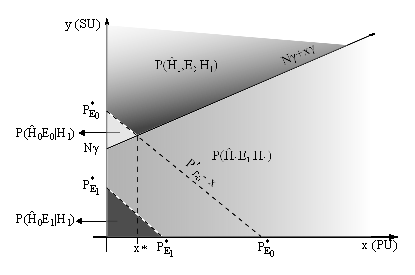
\includegraphics[scale=1.2]{Regions.eps}
\caption{Integration regions to compute the probabilities of correct detection, type I and type II errors under the $H_1$ event (transmission overlap).}\label{fig:Regions}
\end{figure}

Let us now obtain the probabilities for $H_{0}$, i.e. in absence of transmission overlap. The probabilities are defined in the following way
\begin{equation}
\begin{array}{lcl}
\mathbf{P}(\hat{H}_{0},E_{0}|H_{0}) & = & \mathbf{P}\left(\left(P,E\right)\in R_{H_{0}E_{0}}|H_{0}\right)\\
\mathbf{P}(\hat{H}_{1},E_{0}|H_{0}) & = & \mathbf{P}\left(\left(P,E\right)\in R_{H_{1}E_{0}}|H_{0}\right)\\
\mathbf{P}(\hat{H}_{0},E_{1}|H_{0}) & = & \mathbf{P}\left(\left(P,E\right)\in R_{H_{0}E_{1}}|H_{0}\right)\\
\mathbf{P}(\hat{H}_{1},E_{1}|H_{0}) & = & \mathbf{P}\left(\left(P,E\right)\in R_{H_{0}E_{1}}|H_{0}\right)
\end{array}
\end{equation}
We now obtain these probabilities as in the $H_{1}$ case. 
The correct estimation probability $\mathbf{P}(\hat{H}_{0},E_{0}|H_{0})$ is given by
\begin{equation}\label{PH0E0H0}
\begin{array}{lcl}
\mathbf{P}(\hat{H}_{0},E_{0}|H_{0}) & = & \mathbf{P}\left(P\leq p^{*}_{E_{0}},\text{\ttfamily{SINR}}>\gamma|H_{0}\right)\\
& = & \mathbf{P}\left(Y\leq p^{*}_{E_{0}},Y>N\gamma\right)\\
& = & \mathbf{P}\left(N\gamma<Y\leq p^{*}_{E_{0}}\right)\\
& = & \displaystyle\int_{N\gamma}^{p^{*}_{E_{0}}}f_{Y}(y)dy
\end{array}
\end{equation}
which, in the case of Rayleigh fading equals $e^{-N\gamma/p_{ss}}-e^{-p^{*}_{E_{0}}/p_{ss}}$.
The Type I error $\mathbf{P}(\hat{H}_{1},E_{0}|H_{0})$ is 
\begin{equation}\label{PH1E0H0}
\begin{array}{lcl}
\mathbf{P}(\hat{H}_{1},E_{0}|H_{0}) & = & \mathbf{P}\left(P>p^{*}_{E_{0}}, \text{\ttfamily{SINR}}>\gamma|H_{0}\right)\\
& = & \mathbf{P}\left(Y>p^{*}_{E_{0}},Y>N\gamma\right)\\
& = & \mathbf{P}\left(Y>\text{max}\left(p^{*}_{E_{0}},N\gamma\right)\right)\\
& = & \mathbf{P}\left(Y>p^{*}_{E_{0}}\right)\\
& = & \displaystyle\int_{p^{*}_{E_{0}}}^{\infty}f_{Y}(y)dy
\end{array}
\end{equation}
For Rayleigh fading $\mathbf{P}(\hat{H}_{1},E_{0}|H_{0})=e^{-p^{*}_{E_{0}}/p_{ss}}$.
The correct estimation probability at the $E_{1}$ event is
\begin{equation}\label{PH0E1H0}
\begin{array}{lcl}
\mathbf{P}(\hat{H}_{0},E_{1}|H_{0}) & = & \mathbf{P}\left(P\leq p^{*}_{E_{1}}, \text{\ttfamily{SINR}}\leq\gamma|H_{0}\right)\\
& = & \mathbf{P}\left(Y\leq p^{*}_{E_{1}},Y\leq N\gamma\right)\\
& = & \mathbf{P}\left(Y\leq\text{min}\left(N\gamma+X\gamma,p^{*}_{E_{1}}\right)\right)\\
& = & \mathbf{P}\left(Y\leq p^{*}_{E_{1}}\right)\\
& = & \displaystyle\int_{0}^{p^{*}_{E_{1}}}f_{Y}(y)dy
\end{array}
\end{equation}
which for Rayleigh fading is $1-e^{-p^{*}_{E_{1}}/p_{ss}}$. Finally the Type I error probability at the $E_{1}$ event is
\begin{equation}\label{PH1E1H0}
\begin{array}{lcl}
\mathbf{P}(\hat{H}_{1},E_{1}|H_{0}) & = & \mathbf{P}\left(P>p^{*}_{E_{1}}, \text{\ttfamily{SINR}}\leq\gamma|H_{0}\right)\\
& = & \mathbf{P}\left(Y>p^{*}_{E_{1}},Y\leq N\gamma\right)\\
& = & \mathbf{P}\left(p^{*}_{E_{1}}<Y\leq N\gamma\right)\\
& = & \displaystyle\int_{p^{*}_{E_{1}}}^{N\gamma}f_{Y}(y)dy
\end{array}
\end{equation}
which equals $e^{-p^{*}_{E_{1}}/p_{ss}}-e^{-N\gamma/p_{ss}}$ for Rayleigh fading.

\section{Application to OSA}\label{sec:Markov}
\begin{figure}[ht]
\centering
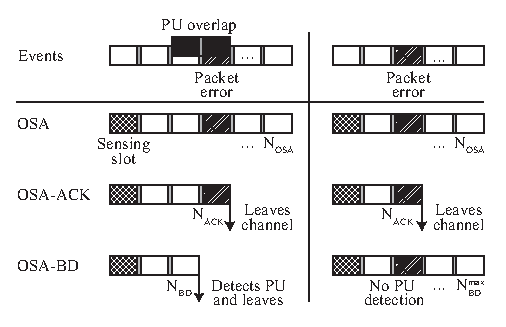
\includegraphics[scale=1]{Slots.eps}
\caption{Transmission periods with an OSA system, an enhanced OSA with an ACK mechanism and our proposal. On the left, how these mechanisms react to a PU overlap that causes a packet error on its second transmission slot. On the right, how these systems react to packet errors without PU presence. Inter-slot periods are required for signaling.}\label{fig:Slots}
\end{figure}

In the following sections, we analyze the use of the proposed background detection (BD) mechanism in an OSA system, studying its effect on the SU throughput and collision probability with PU transmissions, compared to common practical approaches in OSA. 

We assume single-channel transmission capabilities for the SU, leaving for future research the generalization to the multiple-channel case.
We also assume that it takes certain number of slots $n_s$ for the SU to detect at least one available channel. For the sake of simplicity, we will consider $n_s$ fixed to 5, although, as we explain later, the resulting expressions can be easily generalized for the case of a randomly distributed $n_s$.
An SU transmission period consists of these scanning slots followed by a number of consecutive transmission time-slots.
The SU transmits one data packet in each one of these consecutive time-slots.
The PU inter arrival time and the PU channel holding time are characterized by geometric distributions, i.e. the equivalent of a Poisson traffic model for discrete-time. 
In every time-slot, a channel free of PU traffic is occupied by a PU transmission with probability $p$, and an ongoing PU transmission ends with probability $q$.
We can therefore characterize the PU activity in a channel as a two-state discrete time Markov chain (DTMC), whose transition matrix is $M=\left[\begin{smallmatrix}1-p&p\\q&1-q\end{smallmatrix}\right]$.
Considering the $n$-th time-slot of an SU transmission period, $\phi_{n}$ denotes the probability distribution of the DTMC state on this time-slot. In the single-channel traffic model considered, $\phi_{n}$ contains two elements: $\phi_{n}(1)$ and $\phi_{n}(2)$, corresponding to no PU activity and PU activity in the channel respectively. The probability distribution in the scanning slot is $\phi_{0} = (1,0)$ if the detection is perfect. With imperfect sensing, $\phi_{0} = (1-p_{\bar{n}},p_{\bar{n}})$, where $p_{\bar{n}}$ denotes the probability of false negative (the sensing outcome indicates that the channel is free of PU activity when it is not). Given the transition matrix $M$, the probability distribution for the $n$-th time-slot is given by $\phi_{n}' = M^{n}\phi_{n}'$, where ``$'$'' stands for the transpose operation.

Two parameters characterize the \textit{system performance}: the SU \textit{throughput} ($T$), defined as the expected number of correctly received SU packets per time-slot in an SU transmission period, and the \textit{collision probability} $P_{c}$, defined as the PU-SU transmission overlap probability per time-slot in an SU transmission period. These parameters can be computed by means of a Markov reward process characterizing the number of consecutive SU transmission slots.

We compare 3 approaches: A generic optimized OSA, an optimized OSA incorporating ACKs, and our proposal OSA-BD. Let us summarize them.
%Our proposal is compared to two generic approaches: an optimized OSA and OSA-ACK. 

\textbf{OSA.} In (optimized) OSA, the SU transmits in the channel during a fixed number of slots $N_{OSA}$. This number is set to the integer solving
\begin{equation}\label{eq:OSA} 
\begin{array}{ll}
\underset{n}{\mbox{max }} T(n)\\
\mbox{subject to } & P_{c}(n) \leq \alpha \\
& 0 \leq n \leq n^{\text{max}}_{\text{OSA}} 
\end{array}
\end{equation}
% \begin{array}[ll]
% \underset{n}\mbox{max} & T(n)\mbox{,  subject to }P_{c}(n) \leq \alpha \\
% & 0 \leq n \leq n^{\text{max}}_{\text{OSA}} 
% \end{array}
% \end{equation}
where $n^{\text{max}}_{\text{OSA}}$ stands for avoiding unbounded $n$ in case $T(n)$ attains its maximum at $n \rightarrow \infty$ and $P_{c}(n)$ remains under $\alpha$ for every $n$.
Note that, provided that $\phi_{0} = (1,0)$, $P_{c}(n)$ is a monotonically increasing sequence bounded by $p/(p+q)$. If several values of $n$ attain the maximum, the OSA algorithm picks the one with the lowest $P_{c}$. We refer to this value as $N_{\text{OSA}}$.

The expression for $P_{c}(n)$ is given by
\begin{equation}
P_{c}(n) = \displaystyle\frac{1}{n+n_s}\displaystyle\sum_{i=1}^{n}\phi_{i}(2)
\end{equation}

Defining $\mathbf{P}(E_{0}|H_{0})$ as the probability of correctly receiving an SU packet in the absence of collision, and $\mathbf{P}(E_{0}|H_{1})$ as the probability of $E_{0}$ in a time-slot with collision, $T(n)$ is given by the following equation
\begin{equation}
T(n) = \displaystyle\frac{1}{n+n_s}\left[\displaystyle\sum_{i=1}^{n}\phi_{i}(1)\mathbf{P}(E_{0}|H_{0}) + \displaystyle\sum_{i=1}^{n}\phi_{i}(2)\mathbf{P}(E_{0}|H_{1})\right]
\end{equation}
The probability $\mathbf{P}(E_{0}|H_{0})$ is obtained as follows
\begin{equation}\label{PE0H0}
\begin{array}{lcl}
\mathbf{P}(E_{0}|H_{0}) & = & \mathbf{P}\left(\text{\ttfamily{SINR}}>\gamma|H_{0}\right)\\
& = & \mathbf{P}\left(Y>N\gamma\right)\\
& = & \displaystyle\int_{N\gamma}^{\infty}f_{Y}(y)dy
\end{array}
\end{equation}
%The reception error probability under collision is 
and $\mathbf{P}(E_{0}|H_{1})$ is given by
\begin{equation}\label{PE0H1}
\begin{array}{lcl}
\mathbf{P}(E_{0}|H_{1}) & = & \mathbf{P}\left(\text{\ttfamily{SINR}}>\gamma|H_{1}\right)\\
& = & \mathbf{P}\left(Y>N\gamma+X\gamma\right)\\
& = & \displaystyle\int_{0}^{\infty}\displaystyle\int_{N\gamma+x\gamma}^{\infty}f_{Y}(y)f_{X}(x)dydx
\end{array}
\end{equation}
For Rayleigh fading we have 
\begin{equation}
\begin{array}{lcl}
\mathbf{P}(E_{0}|H_{0}) & = & e^{-\frac{N\gamma}{p_{ss}}}\\
\mathbf{P}(E_{0}|H_{1}) & = & \displaystyle\frac{p_{ss}e^{-\frac{N\gamma}{p_{ss}}}}{p_{ss} + p_{ps}\gamma}
\end{array}
\end{equation}
The SU uses estimations of $p$ and $q$ to optimize the duration of the transmission period under collision probability constraints.
In our numerical results we evaluate the impact of the estimation inaccuracies on the performance. 
 
\textbf{OSA-ACK.} With this version of the protocol, when an SU Tx packet is not decoded correctly by the SU Rx, the SU Rx sends a NACK to the SU Tx and vacates the channel, aborting transmission. 
This is the same as assuming that every decoding error is due to collision with a PU. 
Thus, the number of consecutive SU transmission slots, $N_{ACK}$, is a random variable.
We set a maximum number of consecutive transmission slots also for this case, denoted by $N_{ACK}^{max}$.

\textbf{OSA-BD.}
Because BD can detect PU activity simultaneously to SU packet reception, the SU transmission can be aborted at any time-slot.
Thus, the number of consecutive transmission slots, $N_{BD}$, denotes a random variable.
We also determine a maximum value for consecutive transmissions in OSA-BD, denoted by $N^{max}_{BD}$.

Both OSA-ACK and OSA-BD are used on top of an optimized OSA. This implies that $N_{ACK}^{max}$ and $N_{BD}^{max}$ are set to the optimal integer solving (\ref{eq:OSA}) for each mechanism. Note that the underlying Markov process is different for each access strategy.
Fig. \ref{fig:Slots} illustrates the behavior of each scheme. Let us describe the Markov-reward model of the SU transmission process for OSA-BD.
It consists in a discrete-time Markov chain (DTMC) in which each state is associated to a reward defined in terms of $T$ of $P_{c}$, depending on what is being computed.
The DTMC, denoted by $Z_{k}$, characterizes a process of consecutive SU transmissions, where $k$ enumerates time-slots. 
The integer value $i$ taken by $Z_{k}$. i.e. the state of the DTMC at the $k$-th time-slot, has the following interpretation:
\begin{itemize}
	\item If $i$ is odd, the channel is free of PU activity (${H}_{0}$) at the $\left\lceil i/2\right\rceil$-th time-slot.
	\item If $i$ is even, the channel presents PU activity (${H}_{1}$) at the $i/2$-th time-slot.
\end{itemize}
After the scanning time-slot ($i=0$), the SU transmits with probability $1$, and enters state $i=1$ with probability $1-p$ and state $i=2$ with probability $p$.
The DTMC advances to a higher state if the BD does not detect PU activity ($\hat{H}_{0}$), and returns to state 0 otherwise, which means the end of the ongoing SU transmission.
Therefore, the DTMC transition probabilities are defined as
\begin{equation}
\begin{array}{lcll}\label{BD_transition_prob}
p_{0,1} & = & 1-p &\\
p_{0,2} & = & p &\\
p_{2k-1,2k+1} & = & (1-p)\mathbf{P}(\hat{H}_{0}|H_{0}) &,\mbox{ for } 0<k<n\\
p_{2k-1,2k+2} & = & p\mathbf{P}(\hat{H}_{0}|H_{0}) &,\mbox{ for } 0<k<n\\
p_{2k-1,0} & = & 1-\mathbf{P}(\hat{H}_{0}|H_{0}) &,\mbox{ for } 0<k<n\\
p_{2k,2k+1} & = & q\mathbf{P}(\hat{H}_{0}|H_{1}) &,\mbox{ for } 0<k<n\\
p_{2k,2k+2} & = & (1-q)\mathbf{P}(\hat{H}_{0}|H_{1}) &,\mbox{ for } 0<k<n\\
p_{2k,0} & = & 1-\mathbf{P}(\hat{H}_{0}|H_{1}) &,\mbox{ for } 0<k<n\\
p_{n,0} & = & 1 &
\end{array}
\end{equation}
where $\mathbf{P}(\hat{H}_{0}|H_{0})$ and $\mathbf{P}(\hat{H}_{0}|H_{1})$ can be obtained as follows
\begin{equation}
\begin{array}{lcl}
\mathbf{P}(\hat{H}_{0}|H_{0}) & = & \mathbf{P}(\hat{H}_{0},E_{0}|H_{0}) + \mathbf{P}(\hat{H}_{0},E_{1}|H_{0})\\
\mathbf{P}(\hat{H}_{0}|H_{1}) & = & \mathbf{P}(\hat{H}_{0},E_{0}|H_{1}) + \mathbf{P}(\hat{H}_{0},E_{1}|H_{1})
\end{array}
\end{equation}
where $\mathbf{P}(\hat{H}_{0},E_{0}|H_{1})$, $\mathbf{P}(\hat{H}_{0},E_{1}|H_{1})$, $\mathbf{P}(\hat{H}_{0},E_{0}|H_{0})$, and $\mathbf{P}(\hat{H}_{0},E_{1}|H_{0})$, are obtained by (\ref{PH0E0H1}), (\ref{PH0E1H1}), (\ref{PH0E0H0}), and (\ref{PH0E1H0})respectively.
Fig. \ref{fig:Markov} depicts the graph of the DTMC.

\begin{figure}[ht]
\centering
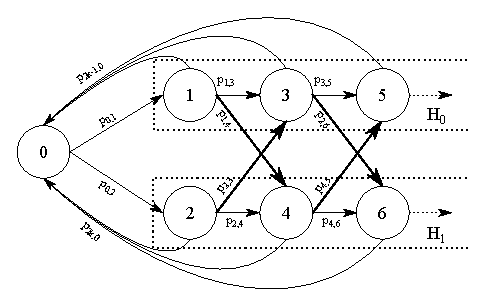
\includegraphics[scale=1]{Markov.eps}
\caption{Graph of the DTMC characterizing the SU transmission process of OSA-BD.}\label{fig:Markov}
\end{figure}

For a generic reward $r(i)$, the expected average reward is defined as 
$\bar{r} = \underset{K\rightarrow\infty}{\text{lim }}\frac{1}{K}\sum_{k = 0}^{K}r\left(Z_{k}\right)$. For an ergodic, finite-state Markov chain, and provided that $\left|r\left(i\right)\right|$ is bounded for every $i$, the total expected average reward $\bar{r}$ is $\bar{r} = \sum_{i = 0}^{n}r\left(i\right)\pi_{i}$, where $\pi_{i}$ are the steady state probabilities of the DTMC obtained by solving the equilibrium equations $\boldsymbol{\pi} = \boldsymbol{\pi}\mathbf{T}$, $\left\|\boldsymbol{\pi}\right\| = \displaystyle\sum_{i=0}^{n}\pi_{i}=1$, where $\mathbf{T}$ is the transition matrix containing the probabilities defined in (\ref{BD_transition_prob}). Let $r_{T}(i)$ and $r_{P_{c}}(i)$ denote the per-state reward for computing $T$ and $P_{c}$ respectively. According to the definitions of $T$ and $P_{c}$, and because the DTMC models consecutive SU transmissions, we have that $\bar{r}_{T} = T$ and $\bar{r}_{P_{c}} = P_{c}$. When using BD, we will use the terms $\bar{r}_{T}(n)$ and $\bar{r}_{P_{c}}(n)$ to refer to the expected averages for the SU throughput and collision probability given a maximum length, $n$, of SU transmissions. The optimal $n$ is obtained by solving the following optimization problem:
\begin{equation}
\underset{n}{\mbox{max }} \bar{r}_{T}(n)\mbox{ subject to }\bar{r}_{P_{c}}(n) \leq \alpha
\end{equation}
which is solved for integers $n \in \left\{0,1,\ldots,n_{\text{m}}\right\}$. 
Note that the trivial values for $n=0$ are $\bar{r}_{T}(0)=0$ and $\bar{r}_{P_{c}}(0)=0$. 
If there is more than one solution, the optimal transmission limit, $n^{*}$, is the lowest one attaining the maximum throughput.

Let us see how to obtain the per-stage reward functions $r_{T}(i)$ and $r_{P_{c}}(i)$, for every $i$. The per-stage throughput $r_{T}(i)$ is defined as the expected number of SU packets correctly received at the $i$-th SU transmission time-slot. By definition, for every $i>0$, the SU transmits one packet, therefore $r_{T}(i) = \mathbf{P}(E_{0}|i)\cdot1$, where $\mathbf{P}(E_{0}|i)$ is the probability of the $E_{0}$ event at the $i$-th time-slot, and is given by
\begin{equation}
\mathbf{P}(E_{0}|i) =
\begin{cases}
\mathbf{P}(E_{0}|H_{0}) &,\mbox{if }i\mbox{ odd}\\
\mathbf{P}(E_{0}|H_{1}) &,\mbox{if }i\mbox{ even}
\end{cases}
\end{equation}
%By applying the law of total probability we have
%\begin{equation}
%\begin{array}{lcl}
%r_{T}(i) & = & \mathbf{P}(E_{0}|i)\\
%& = & \mathbf{P}(E_{0}|H_{0})\mathbf{P}(H_{0}|i) + \mathbf{P}(E_{0}|H_{1})\mathbf{P}(H_{1}|i)\\
%& = & \mathbf{P}(E_{0}|H_{0})\phi_{i}(1) + \mathbf{P}(E_{0}|H_{1})\phi_{i}(2)
%\end{array}
%\end{equation}
for $i>0$, where $\mathbf{P}(E_{0}|H_{0})$ and $\mathbf{P}(E_{0}|H_{1})$ are given by (\ref{PE0H0}) and (\ref{PE0H1}) respectively. Similarly, the per-stage collision probability is $r_{P_{c}}(i)~=~0$ when $i$ is odd, and $r_{P_{c}}(i)~=~1$ when $i$ is even. For $i=0$ we have $r_{T}(0)~=~0$ and $r_{P_{c}}(0)~=~0$. 

The specific structure of matrix $\mathbf{T}$ allows an efficient computation of the steady-state probability vector $\boldsymbol{\pi}$. Let us express $\mathbf{T}$ in a block-matrix form
\begin{equation}
\mathbf{T} =
\begin{pmatrix}
			\mathbf{B}_{0,0} & \mathbf{B}_{0,1}  & \mathbf{0} & \mathbf{0} & \cdots \mathbf{0} \\
			\mathbf{B} & \mathbf{0} & \mathbf{A} & \mathbf{0} & \cdots \mathbf{0} \\
			\mathbf{B} & \mathbf{0} & \mathbf{0} & \mathbf{A} & \cdots \mathbf{0} \\
			\vdots & \vdots & \vdots & \vdots &  \vdots\\
			\mathbf{1} & \mathbf{0} & \mathbf{0} & \mathbf{0} & \cdots \mathbf{A} \\
			\end{pmatrix}
\end{equation}
where $\mathbf{B}_{0,0} = (0, 0)$, $\mathbf{B}_{0,1} = ((1-p), p)$, and
\begin{equation}
\begin{array}{lcl}
\mathbf{A} & = &
\begin{pmatrix}
			(1-p)\mathbf{P}(\hat{H}_{0}|H_{0}) & p\mathbf{P}(\hat{H}_{0}|H_{0})\\
			q\mathbf{P}(\hat{H}_{0}|H_{1}) & (1-q)\mathbf{P}(\hat{H}_{0}|H_{1})\\
			\end{pmatrix}\\
\mathbf{B} & = &
\begin{pmatrix}
			1-\mathbf{P}(\hat{H}_{0}|H_{0})\\
			1-\mathbf{P}(\hat{H}_{0}|H_{1})\\
			\end{pmatrix}\\
\mathbf{1} & = &
\begin{pmatrix}
			1\\
			1\\
			\end{pmatrix}\\			
\end{array}
\end{equation}
Let us define $\boldsymbol{\pi}_{k}~=~(\pi_{2k-1}, \pi_{2k})$, denoting the probability of the events $H_{0}$ and $H_{1}$ at the $k$-th transmission slot. Applying the equilibrium equations we have $\pi_{0}~=~\sum_{k=1}^{n-1}\boldsymbol{\pi}_{j}\mathbf{B} + \boldsymbol{\pi}_{n}\mathbf{1}$, $\boldsymbol{\pi}_{1}~=~\pi_{0}\mathbf{B}_{0,1}$, and $\boldsymbol{\pi}_{k}$ can be expressed in the matrix-geometric form $\boldsymbol{\pi}_{k}~=~\boldsymbol{\pi}_{1}\mathbf{A}^{k-1}~=~\pi_{0}\mathbf{B}_{0,1}\mathbf{A}^{k-1}$, for $k > 1$. The normalization condition is $\pi_{0}+\sum_{k=1}^{n-1}\boldsymbol{\pi}_{j}\mathbf{1} + \boldsymbol{\pi}_{n}\mathbf{1}~=~1$, which combined with the equilibrium equations results in the following expression for $\pi_{0}$
\begin{equation}\label{pi_0_basic}
\pi_{0} = \displaystyle\frac{1}{2+\sum_{k=1}^{n-1}\mathbf{B}_{0,1}\mathbf{A}^{k-1}(\mathbf{1}-\mathbf{B})}
\end{equation}
Because $\mathbf{A}$ is strictly positive we know, by the Perron-Frobenius theorem, that it has one positive eigenvalue, with multiplicity 1, which is strictly higher than all other eigenvalues. Since the dimension of $\mathbf{A}$ is $2\times2$, it has only two eigenvalues and thus we conclude that $\mathbf{A}$ has two distinct eigenvalues, $\lambda_{1}$ and $\lambda_{2}$ (with their corresponding eigenvectors $\mathbf{e}_{1}$ and $\mathbf{e}_{2}$). This implies that $\mathbf{A}$ can be expressed as $\mathbf{A}~=~\mathbf{M}\boldsymbol\Lambda\mathbf{M}^{-1}$ where $\mathbf{M}~=~\left[\mathbf{e}_{1} \mathbf{e}_{2}\right]$ and $\boldsymbol\Lambda$ is a diagonal matrix containing $(\lambda_{1}, \lambda_{2})$ in its diagonal. Then
\begin{equation}
\mathbf{A}^{k-1} = 
\mathbf{M}\begin{pmatrix}
\lambda_{1}^{k-1}&0\\
0&\lambda_{2}^{k-1}
\end{pmatrix}
\mathbf{M}^{-1}
\end{equation}
which allows us to express (\ref{pi_0_basic}) in the following closed form
\begin{equation}
\pi_{0} = \left(2+\mathbf{B}_{0,1}\mathbf{M}
\begin{pmatrix}
\frac{1-\lambda_{1}^{n-1}}{1-\lambda_{1}}&0\\
0&\frac{1-\lambda_{2}^{n-1}}{1-\lambda_{2}}
\end{pmatrix}
\mathbf{M}^{-1}(\mathbf{1}-\mathbf{B})\right)^{-1}
\end{equation}
which enables an efficient computation of $\boldsymbol{\pi}_{k}~=~\pi_{0}\mathbf{B}_{0,1}\mathbf{A}^{k-1}$, for $k = 1,\ldots,n$.

The Markov model for OSA-ACK would be similar, and only requires changing the value of correct detection probability in case of no PU activity and missed detection in case of PU activity to
\begin{equation}
\begin{array}{lcl}
\mathbf{P}(\hat{H}_{0}|H_{0}) & = & \mathbf{P}(E_{0}|H_{0}) \\
\mathbf{P}(\hat{H}_{0}|H_{1}) & = & \mathbf{P}(E_{0}|H_{1})
\end{array}
\end{equation}
respectively. That is to say, as we introduced previously, OSA-ACK assumes that every decoding error is due to collision with a PU, thus, a SU with OSA-ACK goes back to sensing whenever there is a packet error: with probability $1-\mathbf{P}(E_{0}|H_{0}$) in case there is no PU activity, and with probability $1-\mathbf{P}(E_{0}|H_{1})$ in case of PU activity.
\section{Numerical Results}\label{BD_sec_results}
\begin{table}
\begin{tabular}{l r|l r} 
\hline
\textbf{Parameter} & \textbf{Assigned value} & \textbf{Parameter} & \textbf{Assigned value}\\\hline
$p_{ss}$&-72.9 dBm & $\mathbf{P}\left(H_{1}\right)$ & 1/3\\
$p_{ps}$&-70.5 dBm & $p^{*}_{E_{0}}$ & -61.8 dBm\\
$N$&-103 dBm & $p^{*}_{E_{1}}$ & -95.9 dBm\\
$\gamma$& 7 dBm & $\mathbf{P}(\hat{H}_{1}|H_{0})$ & $2.65\cdot10^{-6}$\\
$p, q$ & $10^{-3},2\cdot10^{-3}$ & $\mathbf{P}(\hat{H}_{0}|H_{1})$ & 0.1026\\
\hline
\end{tabular}
\centering
\caption{Parameter setting of the reference scenario used in numerical evaluations}
\label{BD_table_param}
\end{table}
We consider a cognitive pair located within a PU BS cell.
The distance between the PU BS and the SU Rx is $d_{ps}=1000$ m. The PU BS transmission power on each channel, $p_{p}$, is 20 dBm. The transmission antenna height is $h_{t} = 10$ m and the receiver is at $h_{r} = 1.5$ m. The transmission and reception antenna gains are $g_{t} = 4$ dB and $g_{r} = 2$ dB, respectively. With these parameters, the average interference power at the SU receiver due to PU BS transmission is given by the pathloss equation $p_{ps} = \displaystyle\frac{p_{p}(h_{t}h_{r})^2g_{t}g_{r}}{d_{ps}^{-4}}$, which equals -70.5 dBm. Assuming that the SU Tx antenna height and gain are 1.5 m and 4 dB, respectively, and that the distance between SU Tx and the SU Rx is $d_{ss} =250$ m, we obtain $p_{ss} = -72.9$ dBm. Considering a channel bandwidth $B = 2$ MHz, and an SU Rx noise figure equal to 18 dB, the total noise power is $N = -103$ dBm. The cognitive pair transmits at a rate of 2 Mbit/s using BPSK modulation and, as explained in Section \ref{BD_sec_system}, each packet is assumed to arrive correctly if BER$<10^{-3}$, therefore the SINR threshold is $\gamma=7$ dB. The main parameters are summarized in Table \ref{BD_table_param}. We will consider the SU Rx accurately knows these parameters, except when stated otherwise.
%We consider $18$ dB noise figure for the SU Rx.
%, with the main parameters summarized in Table \ref{BD_table_param}, where $p_{ss}$ and $p_{ps}$ are the average powers received from the SU Tx and PU BS respectively. 
%The results are particularized for \textit{Rayleigh} fading.

It is interesting to assess how the performance figures vary with the optimization parameter $n$ (in time-slots), as shown in Fig. \ref{fig:PerformanceVsN}. 
%We can notice one of the main advantages of using a detection mechanism: while $P_{c}$ increases almost linearly with $n$ for optimized OSA, it does not surpass a notably low level when ACK or BD is used. 
%The reason is that OSA-BD can detect PU activity during SU transmission, implying the end of the transmission. 
%The same happens for OSA-ACK, because under these parameters, most PU transmissions cause SU packet errors, while there are few SU reception errors caused by fading. 
%For optimized OSA, larger values of $n$ also imply lower $T$, because transmission overlap also degrades SU performance. 
%Observing this, one can anticipate that the BD implementation will be more robust against parameter estimation inaccuracies than plain optimized OSA. 
Setting the collision probability threshold to $\alpha = 0.025$, the optimal $n$ value for optimized OSA is $N_{OSA} = 49$. 
For OSA-ACK and OSA-BD, $T(n)$ increases monotonically with $n$, while $P_{c}(n)$ remains below 0.025, thus, $n$ is unbounded in eq. (\ref{eq:OSA}). We select $N^{max}_{ACK}=N^{max}_{BD}=100$, which assures $P_{c} < 0.05$ in case of malfunction of these mechanisms.
\begin{figure}[ht]
\centering
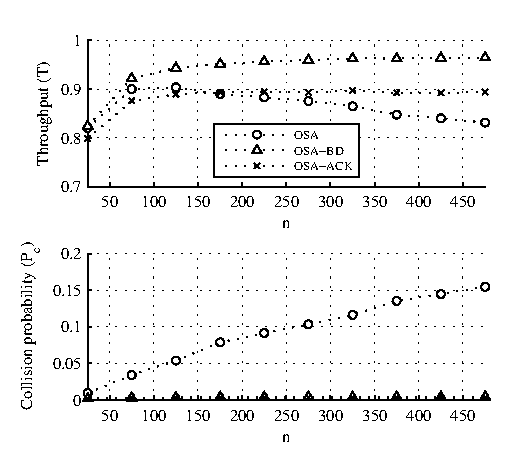
\includegraphics[scale=1]{PerformanceVsN.eps}
\caption[]{Throughput and collision performance with optimized OSA, OSA-ACK and OSA-BD vs. the number of time-slots (n) of the SU transmission. As OSA-ACK and OSA-BD can abort transmissions, their $P_{c}$ remain low.}\label{fig:PerformanceVsN}
\end{figure}

The advantage of the OSA-BD mechanism over OSA-ACK is shown in Fig. \ref{fig:performance_powerRatio}. BD is especially useful compared to the ACK mechanism when $p_{ss}$ is small in relation to $p_{ps}$.
In that case, SU packet errors are caused by propagation issues more often than by PU interference, therefore, the ACK mechanism aborts transmission earlier and attains less throughput per transmission period. 

\begin{figure}[ht]
\centering
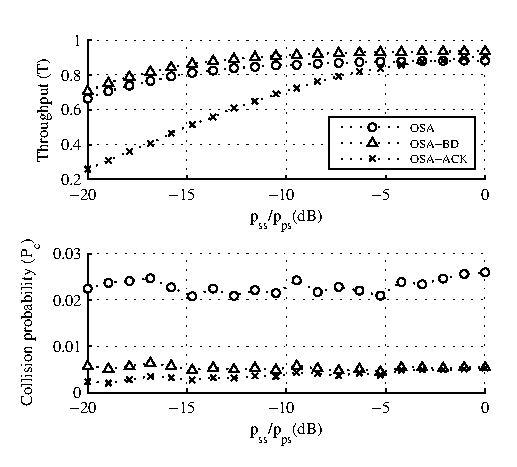
\includegraphics[scale=1]{PerformanceVsPss.eps}
\caption[]{Throughput and collision performance with optimized OSA, OSA-ACK and OSA-BD vs. different ratios of secondary to primary power at the SU receiver. $\alpha = 0.025, N_{OSA} = 49, N_{ACK}^{\text{max}} = N_{BD}^{\text{max}} = 100$.}\label{fig:performance_powerRatio}
\end{figure}


\subsection{Sensitivity to Estimation Inaccuracies}
In this section we evaluate and compare the robustness of OSA, OSA-ACK and OSA-BD.
% under inaccuracies in the estimations of critical parameters. 
%By doing this, we evaluate the robustness of each implementation against inaccuracies on parameter estimations.
Optimized OSA and the BD mechanism are heavily reliant on the characterization of the PU traffic in the channel. 
To evaluate the impact of traffic estimation inaccuracies, let us consider that the arrival traffic intensity $p$ differs from the estimated one, which is used for the computation of $N_{OSA}$ in optimized OSA and for the threshold computation in BD.
In Fig. \ref{fig:pMisestimation} we can see that, in all three systems, $T$ decreases and $P_{c}$ increases but OSA-BD does not suffer a severe degradation and still outpeforms the other two mechanisms.

\begin{figure}[ht]
\centering
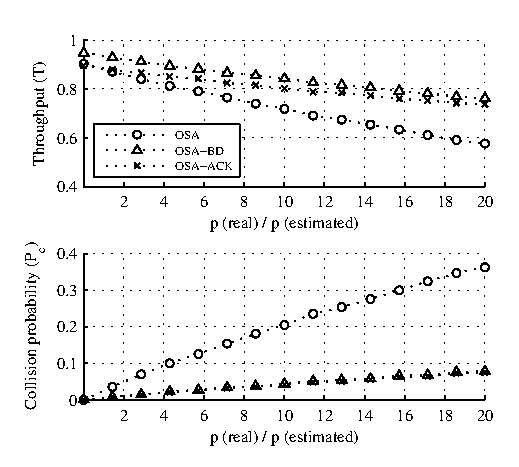
\includegraphics[scale=1]{pMisestimation.eps}
\caption[]{Throughput and collision performance with optimized OSA, OSA-ACK and OSA-BD vs. the inaccuracy on the estimation of the traffic intensity. $\alpha = 0.025, N_{OSA} = 49, N_{ACK}^{\text{max}} = N_{BD}^{\text{max}} = 100$.}\label{fig:pMisestimation}
\end{figure}

Another critical aspect is the channel characterization.
Let us consider that the BD design is based on an errored estimation of the average primary power at the SU Rx, $p_{ps}$.
%The MAP estimator of OSA-BD has been built for Rayleigh fading for both PU and SU signals, assuming previous knowledge of $p_{ps}$ and $p_{ss}$. 
%However it is possible that the SU misestimates the average power, especially $p_{ps}$, or even the channel statistical description itself.
%To assess the effect of these misestimations, 
Fig. \ref{fig:performance_power} shows the performance of each mechanism under different $p_{ps}$ estimation errors, and two types of fading: Rayleigh and Nakagami with $m=2$ (while BD is designed for Rayleigh fading in all cases). 
We see that OSA-BD maintains its advantage with respect to optimized OSA in almost every case, and with respect to OSA-ACK regarding throughput. 
The statistical characterization of the fading shows a moderate impact on BD performance. 
In contrast, overestimating $p_{ps}$ shows a more harmful effect on the collision probability. 
The reason is that, as the real $p_{ps}$ decreases respect the estimated value, the probability of Type II error approaches $1$ and, in consequence the OSA-BD tends to operate as an OSA without BD. 
In Fig. \ref{fig:performance_power}, $N^{max}_{ACK}$ and $N^{max}_{BD}$ are set to $100$ which, as explained previously, results in a $P_{c}$ near 0.05 in case of BD or ACK malfunction.
We can guarantee that the worst-case collision probability of OSA-BD or OSA-ACK is no worse than OSA's, by simply setting $N^{max}_{BD}\leftarrow N_{OSA}$ and $N^{max}_{ACK}\leftarrow N_{OSA}$, respectively.
%If all systems are configured with the same $n^{*}$ value, $N_{OSA} = N^{max}_{ACK} = N^{max}_{BD}$, they show equal worst-case performance.

\begin{figure}[ht]
\centering
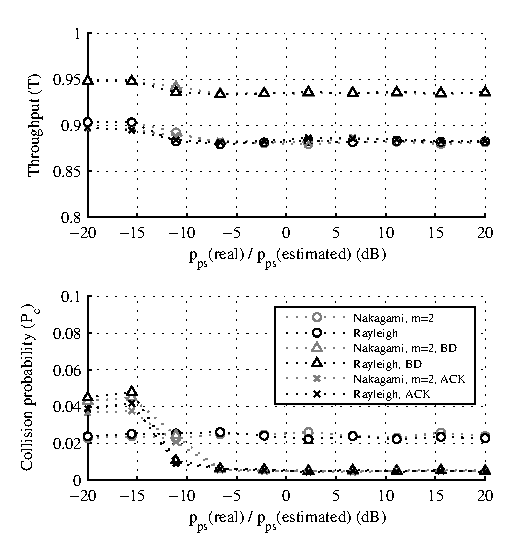
\includegraphics[scale=1]{p_psMisestimationChModel.eps}
\caption[]{Throughput and collision performance with optimized OSA, OSA-ACK and OSA-BD vs. the inaccuracy on the estimation of the primary power received at the SU Rx, for different fading channel characterizations. $\alpha = 0.025, N_{OSA} = 49, N_{ACK}^{\text{max}} = N_{BD}^{\text{max}} = 100$.}\label{fig:performance_power}
\end{figure}


\section{Conclusions}\label{BD_sec_conclusion}
We have considered the problem of interference caused by transmission overlap in OSA. On top of the existing approach of optimized periodic sensing, we have introduced a novel mechanism called Background Detection. This scheme operates at the SU receiver and uses a Maximum \textit{A Posteriori} estimator to decide, upon each SU packet reception, if there has been collision with a PU packet, aborting transmission if necessary. Our results showed that BD allows for longer SU transmission periods, improving SU throughput while reducing collision probability. In addition, although BD is also reliant on traffic estimations, it enhances the robustness of the OSA protocol against estimation inaccuracies, especially in terms of collision probability.
BD shows promising results and it is a simple mechanism to implement (not requiring additional hardware or signaling). 

